\documentclass{beamer}
\usetheme{AnnArbor}
\usepackage{graphicx}
\graphicspath{{pics/}}
\usepackage{amsmath}
\usepackage{amssymb}
\usepackage{framed}
\usepackage{tikz}
\usepackage[]{xcolor}
\usepackage[most]{tcolorbox}
\usepackage{pgfplots}
\pgfplotsset{compat=1.18}
\usepackage{blkarray}
\setbeamercolor{mycolorbox}{%
  bg=yellow!20,   % background color (20% yellow)
  fg=black      % foreground (text) color
}
\usefonttheme[onlymath]{serif}

\newtcolorbox{solutionblock}{
  colback=yellow!5,        % Background color: light yellow
  colframe=orange!80!black, % Frame color: dark orange
  title=Solution,
  fonttitle=\bfseries
}

\title{Introduction to Functions}
\author{Nithin}
\institute{}
\date{\today}
\begin{document}
\begin{frame}
  \titlepage
\end{frame}
\begin{frame}
  \tableofcontents
\end{frame}


\subsection{Domain,Range and Equality}

\begin{frame}
  \frametitle{What is a Function ?}
  \begin{block}{What is a Function?}
    A function associates every number in some set of real numbers, called the domain of the function, with exactly one real number
  \end{block}
\end{frame}



\begin{frame}{Domain}
  \begin{beamercolorbox}[wd=\textwidth,rounded=true,shadow=true]{mycolorbox}
    If a function is defined by a formula, with no domain specified, then the domain is assumed to be the set of all real numbers for which the formula makes sense and produces a real number
  \end{beamercolorbox}
\end{frame}

\begin{frame}{Domain}
  \begin{exampleblock}{Example 3}
    Find the domain of the function \(f\)  defined by \[f (x) = (3x-1)^2 \]
  \end{exampleblock}
  \begin{exampleblock}{Example 4}
    Find the domain of the function \(f\) defined by \[h (t) = \frac{t^2 + 3t + 7}{t-4} \]
  \end{exampleblock}
  \begin{exampleblock}{Example 6}
    Find the domain of the function g defined by \[g(x) = \sqrt{|x|-5}\]
  \end{exampleblock}
\end{frame}
\begin{frame}
  \frametitle{Functions}
  \begin{block}{Range}
    The range of a function \(f\) is the set of all numbers \(y\) such that \(f (x) = y\) for at least one \(x\) in the domain of \(f\)
  \end{block}
%  \begin{figure}[h]
%    \centering
%    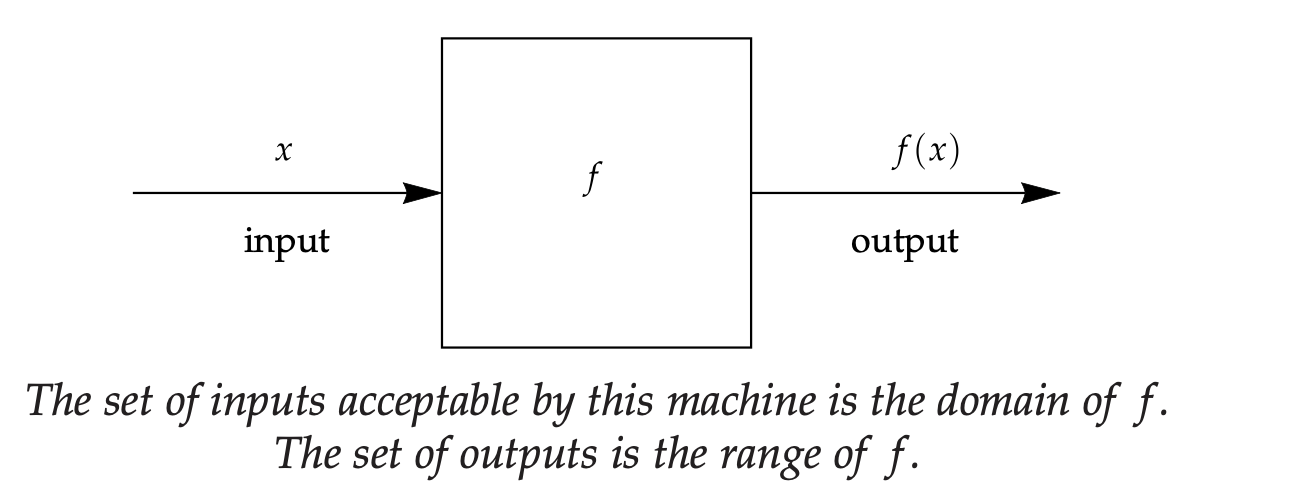
\includegraphics[scale=0.5]{function-engine.png}
%\end{figure}
\end{frame}
\begin{frame}{Functions}
  \begin{exampleblock}{Example 4}
The domain of \(f\) is the interval \( [2, 5] \), with \(f\) defined on this interval by the equation \(f (x) = 3x + 1\)
  \end{exampleblock}
  Solution : \pause 
  \[
  y = f(x) = 3x+1 \]     \pause

  \[  2 \leq \frac{y-1}{3} \leq 5.  \pause
  \]

  \[  7 \leq y \leq 16.   \pause
   \]
\end{frame}
\begin{frame}{Function}
  \begin{exampleblock}{Example 5}
    The domain of \(g\) is the interval \([1,20]\), with \(g\) defined on this interval by
    the equation
    \[
    g(x) = |x - 5|.
    \]
    Is \(2\) in the range of \(g\)?
  \end{exampleblock}
  Solution :  \pause 
  \[ y =  |x-5| \]
  for \(x-5>0 \) ,\(y = x-5 \implies x = y+5 \)  
  \[ 5 < y+5 \leq 20  \implies  0 < y \leq 15 \]
  for \(x-5<0 \), \(y = -(x-5) \implies y = -x+5 \implies 5-y = x \)
  \[ 1 \leq 5-y \leq 5  \implies -4 \leq -y \leq 0 \implies  4 \geq y \geq 0 \] 
\end{frame}
\begin{frame}{Equality of Functions}
  \begin{beamercolorbox}[wd=\textwidth,rounded=true,shadow=true]{mycolorbox}
    Two functions are equal if and only if they have the same domain and the same value at every number in that domain
  \end{beamercolorbox}
  \begin{exampleblock}{Example}
    Suppose \(f\) is the function whose domain is the set of real numbers, with \(f\) defined
    on this domain by
    \[f (x) = x^2\]
    Suppose \(g\) is the function whose domain is the set of positive numbers, with \(g\)
    defined on this domain by
    \[g(x) = x^2\]
    Are \(f\) and \(g\) equal functions ?
  \end{exampleblock}
\end{frame}
\begin{frame}{Equality of functions}
  \begin{exampleblock}{Example 2}
    Suppose \(f\) and \(g\) are functions whose domain is the set consisting of the two numbers \(\{1, 2\}\) with \(f\) and \(g\) defined on this domain by the formulas
\[f (x) = x^2\] and \[g(x) = 3x-2\].Are \(f\) and \(g\) equal functions?
  \end{exampleblock}
\end{frame}
\subsection{Analytical Geometry}
\begin{frame}{What is Analytic Geometry?}
  \begin{itemize}
      \item \textbf{Analytic Geometry} (also called \textit{coordinate geometry} or \textit{Cartesian geometry}) bridges algebra and geometry.
      \item It uses a coordinate system to study geometric shapes and properties.
      \item Geometric objects are represented as algebraic equations.
  \end{itemize}
\end{frame}
\begin{frame}
  \frametitle{Co-ordinate Plane}
  \begin{figure}[h]    
      \centering
      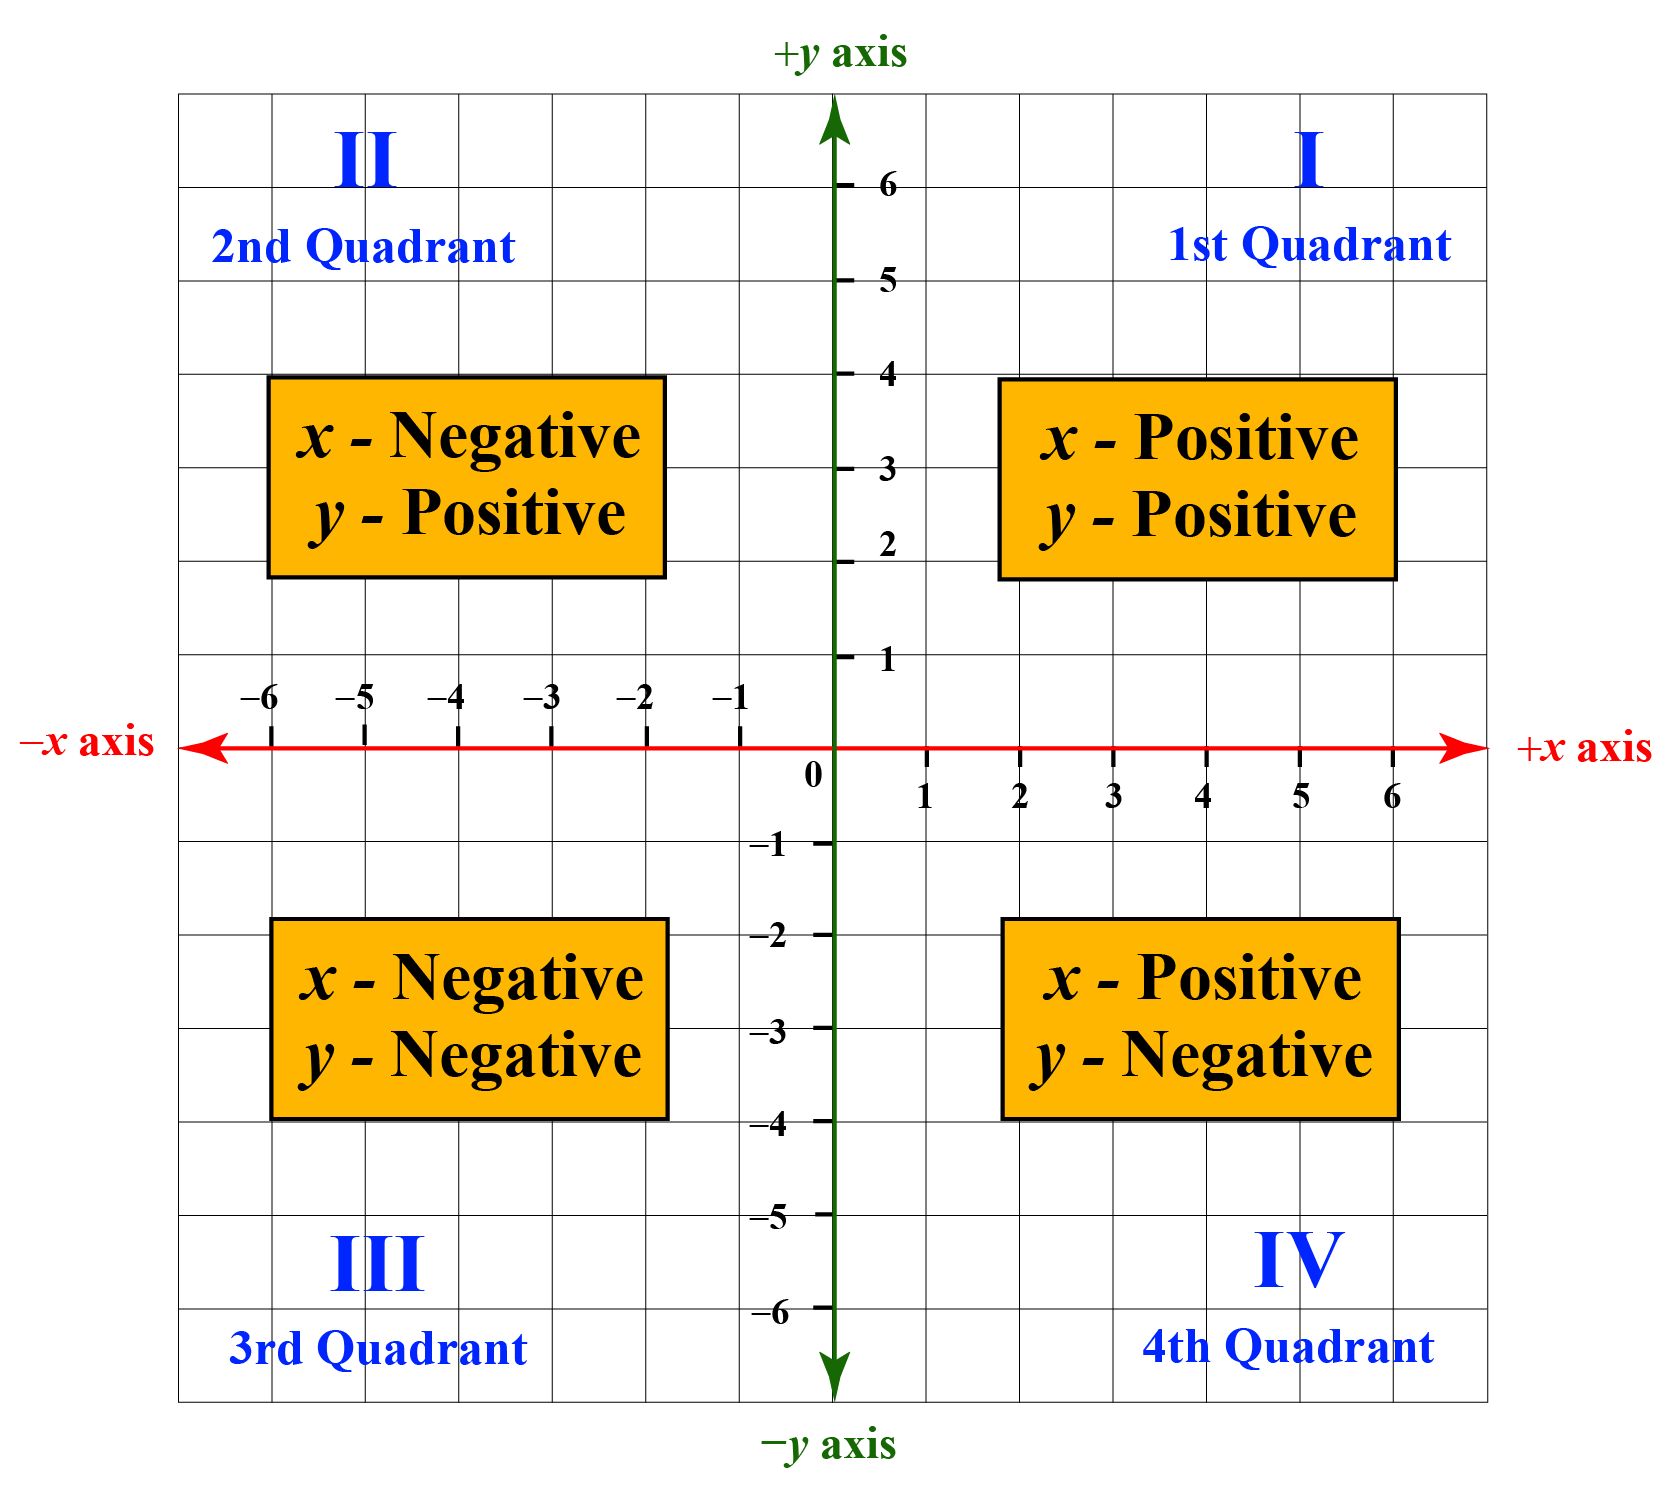
\includegraphics[scale=0.23]{cartesian.png}
\end{figure}
The plane with this system of labeling is often called the \textbf{Cartesian plane} in honor of the French mathematician Rene Descartes(1596-1650), who described this technique in his 1637 book Discourse on Method
\end{frame}
\begin{frame}{Graph Functions}
  \begin{beamercolorbox}[wd=\textwidth,rounded=true,shadow=true]{mycolorbox}
The graph of a function \(f\) is the set of points of the form \(x, f (x)\) as x varies
over the domain of \(f\)
  \end{beamercolorbox}
\end{frame}
\subsubsection{Graphs}
\begin{frame}
  \frametitle{Graph of a Function}
  \begin{figure}[h]    
    \centering
    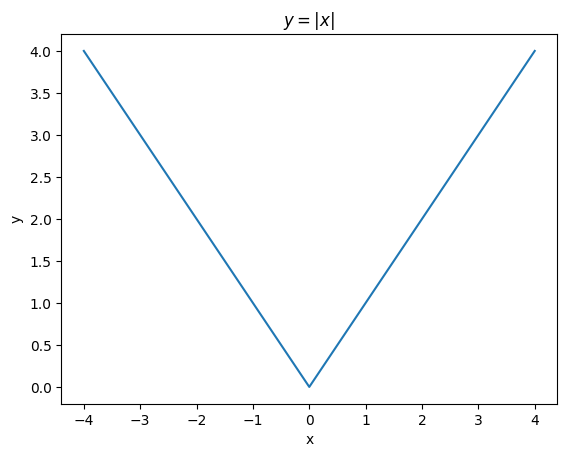
\includegraphics[scale=0.3]{graph.png}
\end{figure}
\begin{figure}[h]    
  \centering
  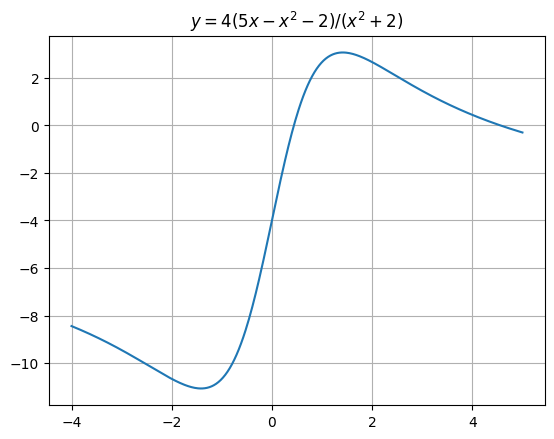
\includegraphics[scale=0.3]{graph2.png}
\end{figure}
\end{frame}

\begin{frame}
  \frametitle{Checking for a function: Vertical line test}
%  \begin{figure}[h]
%  \centering
%  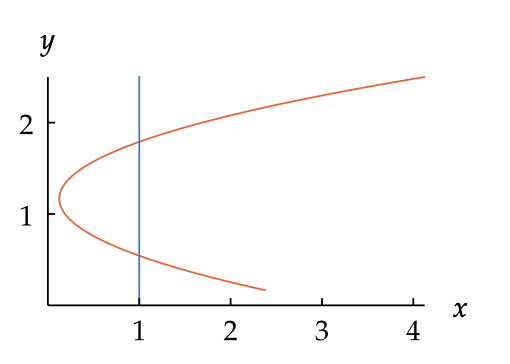
\includegraphics[scale=0.5]{not-fn.png}
%  \end{figure}
  \pause
  The line  \(x=1\) intersects the curve at two points. That is that for each \(x\) value there are multiple \(y\) values which is contradicting to definition of a function 
  \begin{block}{Vertical Line Test}
    A set of points in the coordinate plane is the graph of some function if and only if every vertical line intersects the set in at most one point 
  \end{block}
\end{frame} 
\subsection{Function Transformation}
\begin{frame}
  \frametitle{Vertical Transformations}

  \begin{block}{Shifting a graph up or down}
    Suppose \(f \) is a function and \(a > 0\). Upshift \(g\) and  Downshift \(h\) by
\[g(x) = f (x) + a \;\; h(x) = f (x) - a \]
  \end{block}
  \frametitle{Vertical Transformation}
  \begin{figure}[h]    
    \centering
    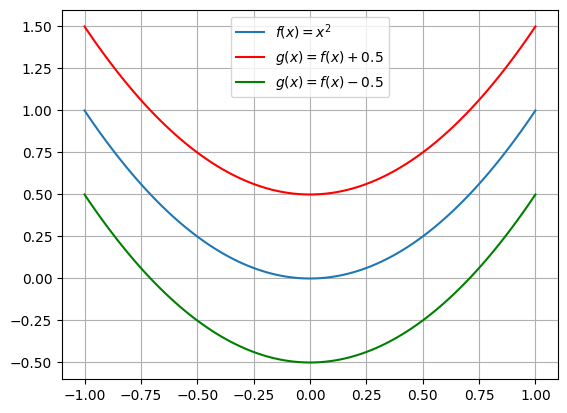
\includegraphics[scale=0.4]{vertical_shift.png}
    \end{figure}
\end{frame}
\begin{frame}
  \frametitle{Vertical Transformation}
  \begin{block}{Vertical Stretch}
    Suppose \(f\) is a function and \(c > 0\). Define a function \(g\) by
\[g(x) = c f (x)\]
  \end{block}
  \begin{figure}[h]    
    \centering
    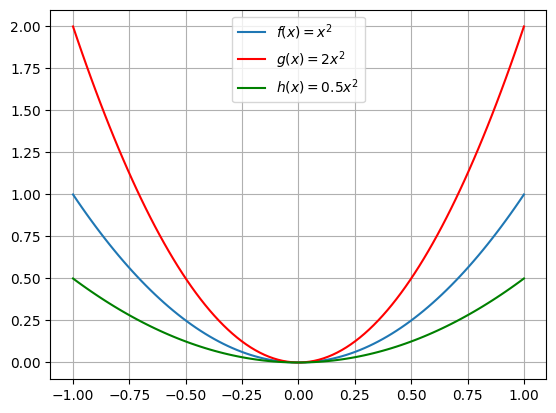
\includegraphics[scale=0.5]{vertical_stretch.png}
    \end{figure}
\end{frame}
\begin{frame}
  \frametitle{Vertical Transformation}
  \begin{block}{Flipping along the Vertical Axis} 
    Vertical fliiping of \(f(x) \) is 
    \[g(x) = - f (x) \]
  \end{block}
  \begin{figure}[h]    
    \centering
    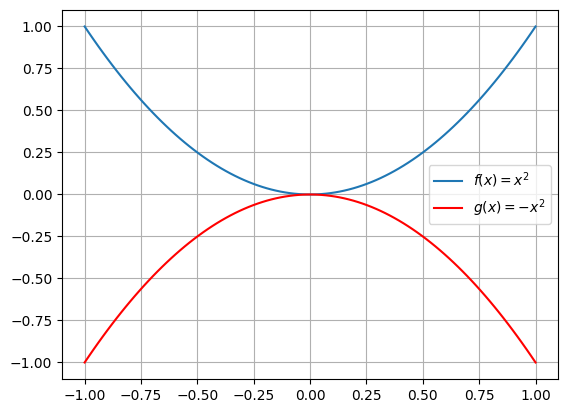
\includegraphics[scale=0.5]{vertical_flip.png}
    \end{figure}
\end{frame}
\begin{frame}
  \frametitle{Horizontal Transformation}
  \begin{block}{Horizontal Shift}
    \[g(x) = f(x+a), h(x) = f(x-a)\]
  \end{block}
  \begin{figure}[h]    
    \centering
    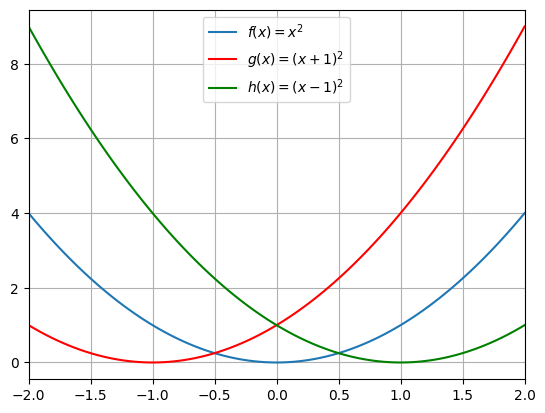
\includegraphics[scale=0.5]{horizontal-shift.png}
    \end{figure}
  \end{frame}
\begin{frame}
    \frametitle{Horizontal Transformation}
    \begin{block}{Horizontal Stretching}
      \[g(x) = f(cx)\]
    \end{block}
    \begin{figure}[h]    
      \centering
      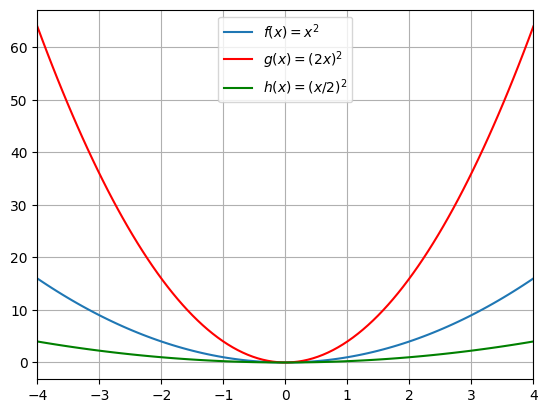
\includegraphics[scale=0.55]{horizontal-stretch.png}
      \end{figure}
\end{frame}
\begin{frame}
  \frametitle{Flipping ac the Vertical Axis}
  \begin{block}{Horizontal Stretching}
    \[g(x) = f(-x)\]
  \end{block}
  \begin{figure}[h]    
    \centering
    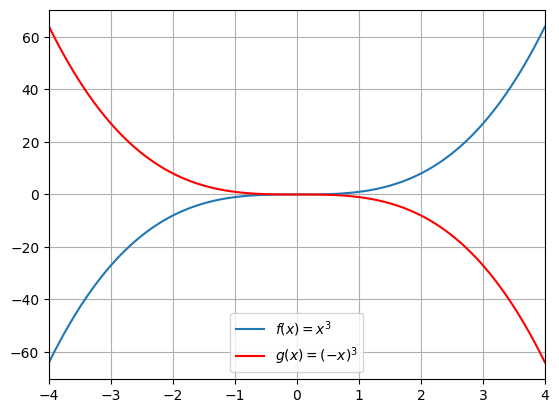
\includegraphics[scale=0.55]{vertical-axis-flip.png}
    \end{figure}
\end{frame}
\begin{frame}
  \frametitle{Combinations of vertical Transformation}
  \begin{figure}[h]    
    \centering
    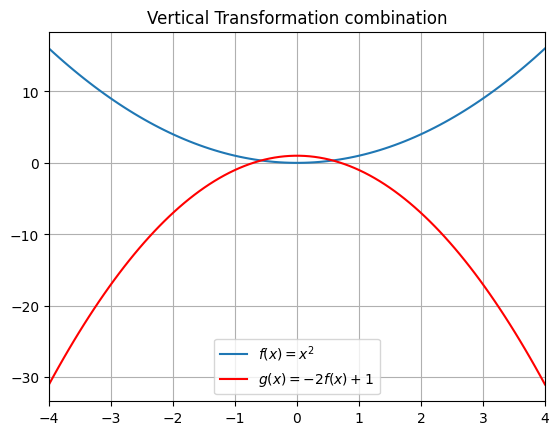
\includegraphics[scale=0.55]{vertical_combination.png}
    \end{figure}
\end{frame}
\begin{frame}{Even Functions}  
\begin{block}{Even}
        \[
        f(-x) = f(x) \quad \text{for all } x \text{ in the domain}
        \]
        Example: \( f(x) = x^2, \quad f(x) = \cos x \)
\end{block}
The graph of an even function is symmetric across the vertical axis 
\end{frame}
\begin{frame}
  \frametitle{Even Functions}
  \begin{columns}
    \column{0.5\textwidth}
    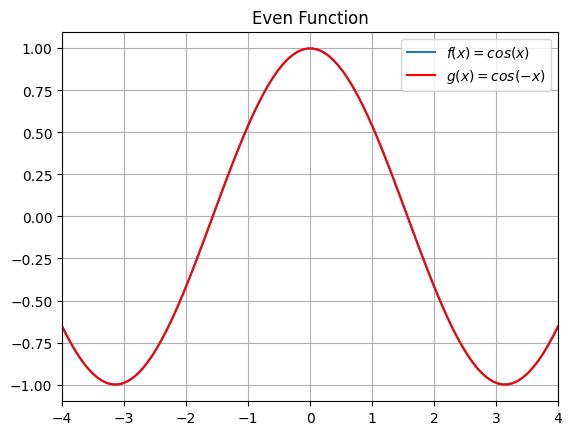
\includegraphics[width=\linewidth]{even.png}

    \column{0.5\textwidth}
    \centering
    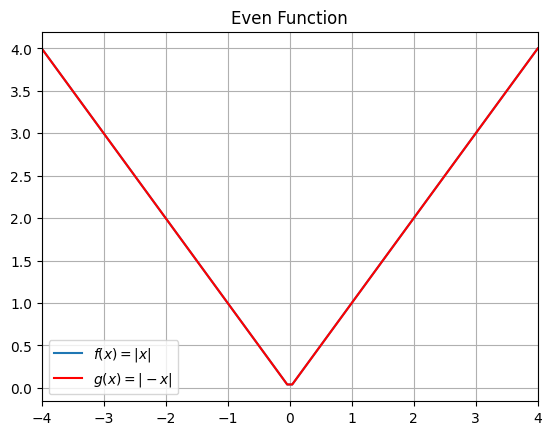
\includegraphics[width=\linewidth]{even2.png}
\end{columns}
\end{frame}
\begin{frame}{Odd Function}
\begin{block}{Odd}
        \[
        f(-x) = -f(x) \quad \text{for all } x \text{ in the domain}
        \]
        Example: \( f(x) = x^3, \quad f(x) = \sin x \)
\end{block}
The graph of an even function is symmetric if flipped or rotated 18 across the origin 
\end{frame}

\begin{frame}
  \frametitle{Odd Function}
  \begin{columns}[T]
    \begin{column}{0.5\textwidth}
    \begin{figure}[t]
    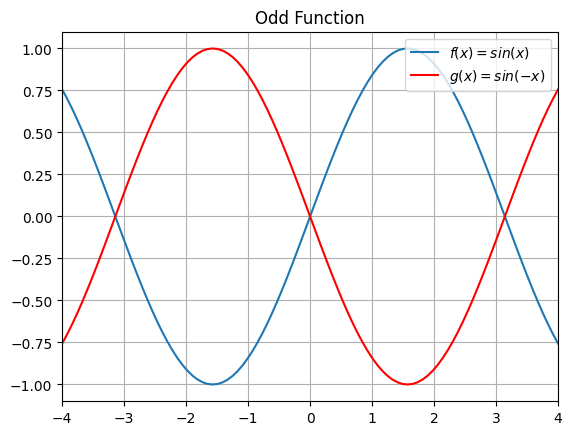
\includegraphics[width=\linewidth]{odd.png}
    \end{figure}
  \end{column}

  \begin{column}{0.5\textwidth}
    \begin{figure}[t]
    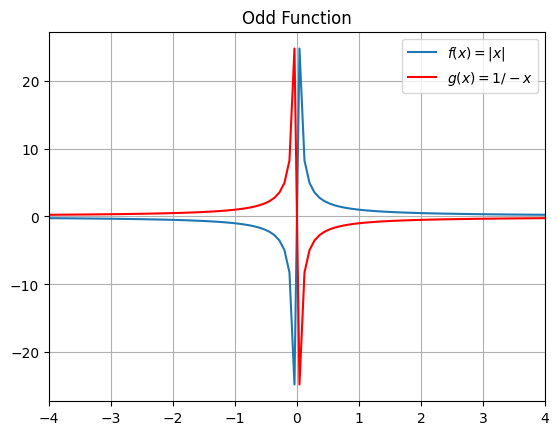
\includegraphics[width=\linewidth]{odd2.png}
    \end{figure}
  \end{column}
\end{columns}
\end{frame}

\subsection{Function Composition}
\begin{frame}
  \frametitle{Algebra of Functions} 
    Suppose \(f\) and \(g\) are functions. We can define new functions from \(f\) and \(g\) as follows: \\
  
  \pause
    \textbf{Sum:}  
    \[
    (f+g)(x) = f(x) + g(x)
    \]
    
    \pause
    \textbf{Difference:}  
    \[
    (f-g)(x) = f(x) - g(x)
    \]
    
    \pause
    \textbf{Product:}  
    \[
    (f\cdot g)(x) = f(x) \cdot g(x)
    \]
    
    \pause
    \textbf{Quotient:}  
    \[
    \left(\frac{f}{g}\right)(x) = \frac{f(x)}{g(x)} \quad \text{provided } g(x) \neq 0.
    \]
    \textbf{Note:} If \(f\) and \(g\) have domains \(D_f\) and \(D_g\), then these operations are defined on the intersection \(D_f \cap D_g\). In the case of the quotient, it is defined on
    \[
    \{x \in D_f \cap D_g : g(x) \neq 0\}.
    \]
    
  \end{frame}

  \begin{frame}
    \frametitle{Exercise }
    \( f(x)  = \sqrt{x-3}\) and \(g(x) = \sqrt{8 - x }\)
    
    Evaluate
    \begin{enumerate}
      \item[a.] \((f+g)(x)\)  
      \item[b.]  \((fg)(x)\)
      \item[c.] Find the domain of above 
    \end{enumerate}
  \pause 
  Sol: 
  \begin{enumerate}
    \item[a.] \(\sqrt{x-3} + \sqrt{8-x} \) 
    \item[b.] \(\sqrt{(x-3)(8-x)} \)  
    \item[c.]  Domian of \begin{enumerate}
      \item[a.] \(x\geq 3 \)  
      \item[b.] \(x \leq 8 \)  
      \item[c.] \( 3 \leq x \leq 8 \)    
    \end{enumerate}
  \end{enumerate}
\end{frame}
  \begin{frame}{Function Composition }
    \begin{block}{Definition:}  
    If \( f(x) \) and \( g(x) \) are functions, then the composition of \( f \) and \( g \), denoted by \( f \circ g \), is defined by
    \[
      (f \circ g)(x) = f(g(x)).
    \]
    \end{block}
    \medskip
    
    \textbf{Example:}
    Consider the function
    \[
      h(x) = \sqrt{x+3}.
    \]
    We can express \( h(x) \) as a composition of two functions \( f \) and \( g \) where:
    \[
      f(x) = \sqrt{x} \quad \text{and} \quad g(x) = x+3.
    \]
    
    Then,
    \[
      h(x) = f(g(x)) = f(x+3) = \sqrt{x+3}.
    \]
  \end{frame}
\begin{frame}
  \frametitle{Exercise}
  \(
  f(x) = \frac{1}{x-4} 
  \) and \( g(x) = x^{2} \) 
  \begin{enumerate}
    \item \(f \circ g \)  
    \item \( g \circ f \)   
    \item domian of \(f \circ g \) 
    \item domain of \( g \circ f \) 
  \end{enumerate}
  Sol: \pause 
  \begin{enumerate}
    \item  \(f(g(x)) = \frac{1}{x^{2} - 4}\)
    \item \(g(f(x)) = (\frac{1}{x-4})^{2}\) 
    \item \(R - \{-2,2\} \)  
    \item \(R - \{4\} \)  
  \end{enumerate}
\end{frame}
\begin{frame}
  \frametitle{Composition Machine}
\begin{figure}
  \centering 
  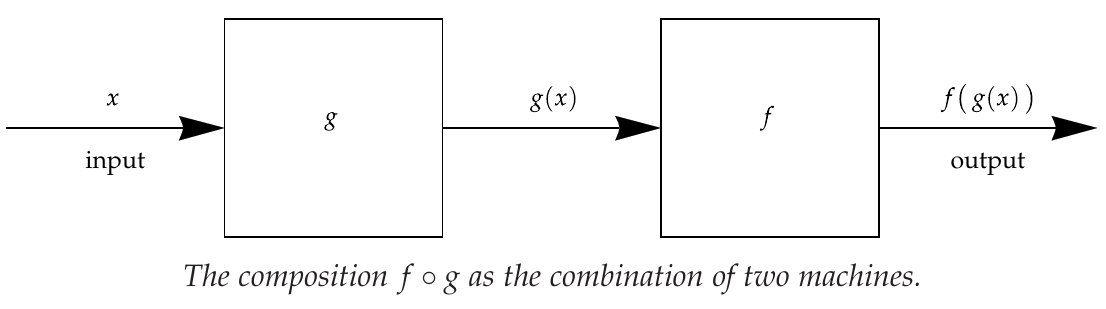
\includegraphics[scale=0.3]{composition.png}
\end{figure}
\end{frame}
\begin{frame}{Excersise}
  \textbf{Problem:} Suppose your cell phone company charges \$0.05 per minute plus \$0.47 for each call to China.
  \begin{enumerate}
    \item[(a)] Find a function \(p\) that gives the amount charged by your cell phone company for a call to China as a function of the number of minutes \(m\).
    \item[(b)] Suppose the tax on cell phone bills is 6\% plus \$0.01 for each call. Find a function \(t\) that gives your total cost, including tax, for a call to China as a function of the amount charged by your cell phone company.
    \item[(c)] Explain why the composition \(t \circ p\) gives your total cost, including tax, of making a cell phone call to China as a function of the number of minutes.
    \item[(d)] Compute a formula for \(t \circ p\).
    \item[(e)] What is your total cost for a ten-minute call to China?
  \end{enumerate}
  \end{frame} 
  \begin{frame}
    \frametitle{Solution}
    
    \textbf{(a)} The company charges \$0.05 per minute plus a fixed charge of \$0.47 per call. Hence, the pre-tax charge function is
    \[
    p(m)=0.05m+0.47.
    \]
    
    \textbf{(b)} The tax on the cell phone bill is 6\% of the pre-tax amount plus an additional \$0.01 per call. Thus, if the pre-tax charge is \(x\), the total cost function (including tax) is
    \[
    t(x)=1.06x+0.01.
    \]
    
    \textbf{(c)} The composition \(t \circ p\) means we first compute the pre-tax charge \(p(m)\) for a call of \(m\) minutes, and then we apply the tax function \(t\) to this amount. In other words, \(t(p(m))\) gives the total cost, including tax, as a function of the number of minutes.
    
    
    \textbf{(d)} To compute the composition, substitute \(p(m)\) into \(t\):
    \[
    (t \circ p)(m)=t(p(m))=1.06\bigl(0.05m+0.47\bigr)+0.01.
    \]
  \end{frame}
  \begin{frame}
    \frametitle{Solution}
    Distribute \(1.06\):
    \[
    1.06(0.05m)=0.053m \quad \text{and} \quad 1.06(0.47)=0.4982.
    \]
    Thus,
    \[
    (t \circ p)(m)=0.053m+0.4982+0.01=0.053m+0.5082.
    \]
    \textbf{(e)} For a ten-minute call (\(m=10\)):
    \[
    (t \circ p)(10)=0.053(10)+0.5082=0.53+0.5082=1.0382.
    \]
    Rounded to the nearest cent, the total cost is approximately \$1.04.
  \end{frame}
  \begin{frame}
    \frametitle{}
    \begin{block}{Identity Function}
      The identity function is defined by
      \[
      I(x) = x \quad \text{for every number } x.
      \]
      \end{block}

      \begin{alertblock}{The function \(I\) is the identity for composition}
        If \(f\) is any function, then
        \[
        f \circ I = I \circ f = f.
        \]
        \end{alertblock}
  \end{frame}
\begin{frame}
  \frametitle{Decomposing the Functions}
  \begin{exampleblock}{Function Decomposition}
    \[
    T(y) = \frac{|y^{2} -3|}{|y^{2} - 7|}
    \]
    Sol: \pause
    \medskip 
    \[f(y) = |y|, g(y) = \frac{y^{2}-3}{y^{2}-7} \]
    \[ f(y) = \frac{|y-3|}{|y-7|}, g(y) = y^{2}\]
  \end{exampleblock}
  \begin{alertblock}{Composition is associative}
    if \(f,g, h\) are functions then 
    \[(f \circ g) \circ h  = f \circ (g \circ h) \]
  \end{alertblock}
\end{frame}
\begin{frame}
  \frametitle{Example}
  \begin{exampleblock}{Composition of three functions}

    \[T(x) = \left| \frac{x^{2}-3}{x^{2} - 7}  \right| \]

    Sol: \pause
     \[f(x) = |x|, g(x) = \frac{x-3}{x-7}, h(x) = x^{2}\]
    
  \end{exampleblock}
\end{frame}
\begin{frame}
  \frametitle{Linear Functions}
  \begin{block}{Linear Function}
    A linear function is a function \(h\) of the form 
    \[h(x) = mx + b\]
    where \(m\) and \(b\) are numbers
  \end{block}
\end{frame}

\begin{frame}
  \frametitle{Linear Functions as Composition}
  \begin{exampleblock}{Vertical Transformations as Compositions}
    A funtion \(g(x)\) is defined by 
    \[g(x)= -2f(x)+1\] 
    Write \(g(x)\) as a the composition of a linear function with \(f(x)\) 
    \[h(x) = -2x + 1 \]
    \[\implies g(x) = h(f(x)) \implies g = h \circ f \]
   \end{exampleblock}
  \end{frame}
  \begin{frame}{Linear Function as Composition}
   \begin{exampleblock}{Horizontal Transformations as Compositions}
    A funtion \(g(x)\) is defined by 
    \[g(x)= f(2x)+1\] 
    Write \(g(x)\) as a the composition of a linear function,  \(f(x)\) and other linear function 
    \[h(x) = x + 1, p(x) = 2x \]
    \[\implies g(x) = h(f(p(x))) \implies g = h \circ f \circ p \]
   \end{exampleblock}
\end{frame}
\subsection{Inverse Functions}
  \begin{frame}
    \frametitle{Inverse Function: Example}
      Consider the function \( f: \mathbb{R} \to \mathbb{R} \) defined by
      \[
      y = \frac{9}{5}x + 32,
      \]
      which converts a temperature \( x \) in Celsius to Fahrenheit \( y \).
      The inverse function \( f^{-1} \) converts Fahrenheit back to Celsius:
      \[
      f^{-1}(y) = \frac{5}{9}(y - 32).
      \]
      Verifying that these functions are inverses:
      \[
      f^{-1}(f(x)) = \frac{5}{9}\Bigl(\frac{9}{5}x + 32 - 32\Bigr) = x,
      \]
      \[
      f(f^{-1}(f)) = \frac{9}{5}\Bigl(\frac{5}{9}(y - 32)\Bigr) + 32 = y.
      \]
  \end{frame}
\begin{frame}
  \frametitle{One-to-One Function}
  \begin{block}{One-to-One Function}
    A function \(f\) is called one-to-one if for each number \(y\) in the range of \(f\) there is
  exactly one number \(x\) in the domain of \(f\) such that \(f (x) = y\)
  \end{block}
\end{frame}

\begin{frame}
  \frametitle{Inverse Function}
  \begin{block}{Definition}
    Suppose \( f \) is a one-to-one function.
    \begin{itemize}
      \item If \( y \) is in the range of \( f \), then \( f^{-1}(y) \) is defined to be the number \( x \) such that \( f(x) = y \).
      \item The function \( f^{-1} \) is called the \emph{inverse function} of \( f \).
    \end{itemize}
    \vspace{1em}
    \textbf{Short version:}
    \begin{itemize}
      \item \( f^{-1}(y) = x \) means \( f(x) = y \).
    \end{itemize}
    \end{block}
\end{frame}
\begin{frame}
  \frametitle{Inverse Function}
\begin{figure}
  \centering
  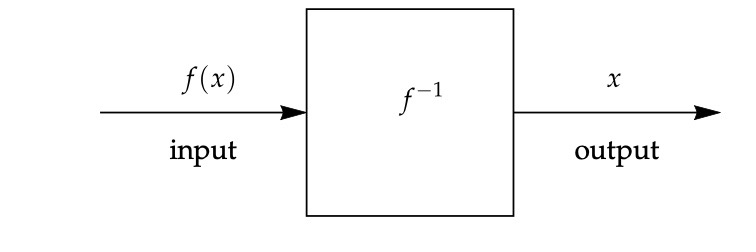
\includegraphics[scale=0.4]{inverse.jpeg}
\end{figure}
\end{frame}
\begin{frame}{Domain and Range of an Inverse Function}
  \begin{block}{Properties}
  If \( f \) is a one-to-one function, then:
  \begin{itemize}
    \item The domain of \( f^{-1} \) equals the range of \( f \).
    \item The range of \( f^{-1} \) equals the domain of \( f \).
  \end{itemize}
  \end{block}
  \end{frame}
  \begin{frame}
    \frametitle{Increasing and Decreasing Function}
    \begin{block}{Increasing}
      A function \(f\) is called increasing if \(f (a) < f (b)\) whenever \(a < b\) and \(a, b \) are in
the domain of \(f\)
    \end{block}
    \begin{block}{Decreasing}
      A function \(f\) is called decreasing if \(f (a) >  f (b)\) whenever \(a < b\) and \(a, b \) are in
the domain of \(f\)
    \end{block}
    \begin{alertblock}{Increasing and decreasing functions are one-to-one}
      \begin{itemize}
        \item Every increasing function is one-to-one
        \item Every decreasing function is one-to-one.
      \end{itemize}
    \end{alertblock}
  \end{frame}
  \begin{frame}
    \frametitle{Exercise}
    \begin{figure}
      \centering
      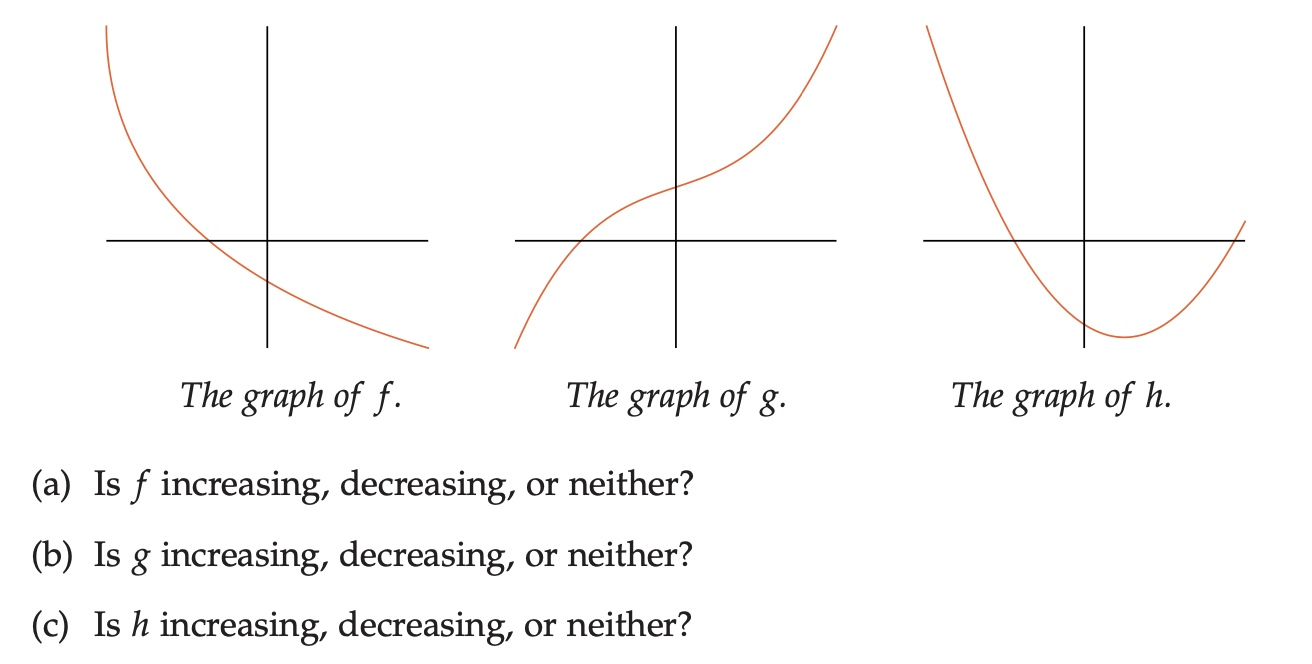
\includegraphics[scale=0.2]{increase.jpeg}
    \end{figure}
    \pause
  \begin{enumerate}
    \item[a.] Decreasing
    \item[b.] Increasing
    \item[c.] Neither
  \end{enumerate}
  \end{frame}
  \begin{frame}
    \frametitle{Do all one-to-one maps are increasing or decreasing ? }
%    \begin{figure}
%      \centering
%      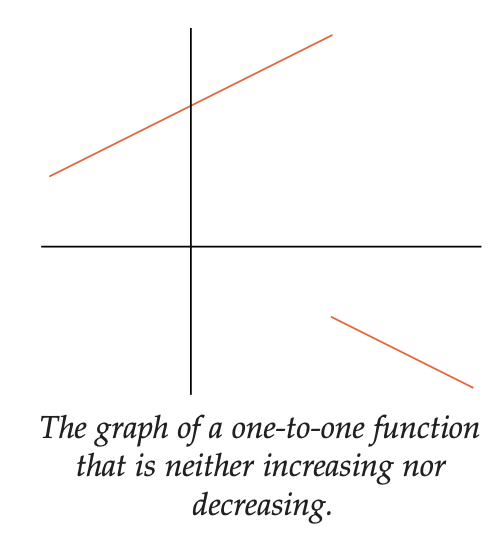
\includegraphics[scale=0.6]{non-increse-decrese.png}
%    \end{figure}
  \end{frame}
  \begin{frame}{Increasing and Decreasing Functions}

    \begin{alertblock}{Inverses of increasing and decreasing functions}
      \begin{itemize}
        \item The inverse of an increasing function is increasing.
        \item The inverse of a decreasing function is decreasing.
      \end{itemize}
    \end{alertblock}
  \end{frame}

\end{document}
  